% Rafael Sartori M. dos Santos, 186154
\documentclass[brazilian,a4paper,twocolumn]{article}

% Título
\title{MC920 -- Trabalho 3}
\author{Rafael Sartori M. Santos, 186154}
\date{17 de outubro de 2019}

% Configuração do documento
\setlength{\parskip}{3pt}
\usepackage[utf8]{inputenc} % tipo de documento UTF-8
\usepackage{mathtools} % permitir expressões matemáticas
\usepackage{breqn} % equações quebradas em várias linhas automaticamente
\usepackage{babel} % configuração da lingua portuguesa
\usepackage{caption} % para legenda de tabelas e figuras
\usepackage[
    pdfauthor={Rafael Sartori M. Santos},
    pdftitle={Trabalho 3 -- MC920},
    pdfproducer={LaTeX (texlive) com hyperref},
    hidelinks
]{hyperref} % para links externos (href)
\usepackage{cleveref} % para referenciar tabelas e figuras melhor
\usepackage{indentfirst} % indentação de todo primeiro parágrafo
\usepackage{graphicx} % para adicionar imagens
\graphicspath{{../imgs/}} % atalho para o caminho das imagens
\usepackage{float} % para fixar posição de imagens
\usepackage{subcaption} % para imagens ficarem lado a lado
% Usamos geometry pois dá mais espaço que fullpage
%\usepackage{geometry} % alterar geometria do papel
%\geometry{a4paper,left=1.7cm,right=1.7cm,top=1cm,bottom=2.0cm} % menor margem
\usepackage{fullpage} % utilizamos uma versão com menos espaçamento nas bordas
\usepackage{verbatim} % pacote para incluir arquivos em verbatim
\usepackage{mdframed} % para enquadrar coisas

% Início do documento
\begin{document}

\maketitle


\section{Introdução}

    O objetivo deste trabalho é separar, rotular, contar objetos desconexos, verificar propriedades, como área, perímetro, centroide, isolar contorno e, por fim, classificá-los entre pequenos, médios e grandes pela área ocupada.

    Faremos isso utilizando um programa escrito em \emph{Python} utilizando a biblioteca padrão, \href{https://opencv.org/}{\emph{OpenCV}}, \href{https://numpy.org/}{\emph{NumPy}} e \href{https://scikit-image.org/}{\emph{scikit-image}} para processar as imagens e \href{https://matplotlib.org/}{\emph{Matplotlib}} para histograma da área calculada dos objetos da imagem.


\section{Método}

    O trabalho é facilmente divisível em várias etapas. Para cumprir todos os objetivos, será necessário:
    \begin{itemize}
        \item monocromatizar a imagem de entrada,
        \item rotular objetos desconexos,
        \item contá-los,
        \item extrair propriedades,
        \item isolar contorno,
        \item classificá-los quanto à área.
    \end{itemize}

    A razão para aplicação de cada um desses passos será explicada junto com sua metodologia mais detalhada. Utilizaremos 3 imagens coloridas fornecidas pelo professor, composta por algumas figuras geométricas bem definidas.

    Para a aplicação de fato, no entanto, iremos utilizar funções já implementadas de \emph{OpenCV} e \emph{scikit-image}, já que seus funcionamentos não diferem tanto dos métodos descritos nesta seção.

    Algumas das funções requerem o tratamento dos resultados de outra função, já que nem sempre são compatíveis.

    \subsection{Monocromatização}

        Como a imagem de entrada é colorida, teremos mais de uma camada de cor e isso tornará difícil a identificação de um objeto ou fundo, as bibliotecas nas funções que utilizaremos recebem apenas uma matriz bidimensional (imagem de camada única). Portanto, qualquer tipo de transformação que produza uma imagem de camada única a partir de várias camadas é suficiente.

        Na aplicação, abrimos a imagem em modo de escala de cinza através da \textit{flag} de \texttt{imread} em \emph{OpenCV}.

    \subsection{Rotulação e contagem}
    \label{sec:metodo-rotulacao}

        Com a imagem monocromática, podemos identificar os objetos através do agrupamento usando \texttt{vizinhança-4} ou \texttt{vizinhança-8}. Podemos fazer isso seguindo este plano:
        \begin{itemize}
            \item inicializamos uma variável que é o número do objeto que estamos identificando atualmente (começa com zero);
            \item inicializamos a matriz de ``resposta'' de mesma dimensão que a entrada com zero (ela guardará o rótulo e quais pontos pertencem a esse objeto);
            \item percorremos a imagem toda; ao encontrarmos um objeto (ponto desconexo em relação ao que estamos -- por exemplo, através de uma cor diferente), fazemos:
            \begin{itemize}
                \item incrementamos a variável do objeto que estamos identificando, esse é o número do objeto atual;
                \item navegaremos dentro dele utilizando a vizinhança selecionada, marcando numa matriz de ``resposta'' o número do objeto atual;
                \item ao não possuir mais pontos que não são fundo alcançáveis pela vizinhança, continuamos percorrendo a imagem.
            \end{itemize}
            \item terminamos a imagem tendo percorrido todos os pontos e rotulado todos os objetos desconexos entre si.
        \end{itemize}

        Dessa forma, automaticamente já contamos os objetos presentes (o valor final da variável do número de objetos que identificamos) e temos uma matriz que possui todos os pontos de cada objeto.

        Com essa matriz, será possível contar a área, identificar perímetro, encontrar centroide e contorno de cada objeto.

        Essa etapa é realizada pelo \emph{scikit-image} através da função \texttt{label}, que identifica e rotula objetos desconexos dada uma vizinhança.

    \subsection{Medir área}
    \label{sec:metodo-area}

        Do resultado do método anterior (\ref{sec:metodo-rotulacao}), podemos medir a área simplesmente contando os pontos que possuem mesmo valor ao rótulo do objeto. Por exemplo, para o rótulo 4, contamos os pontos cujo valor é 4 na matriz retornada.

        Esse algoritmo é implementado pela função \texttt{getprops} (utilizando a rotulação anterior) do \emph{scikit-image}, que também produz outras propriedades.

    \subsection{Isolar contorno e medir perímetro}

        Do resultado da \cref{sec:metodo-rotulacao}, podemos isolar cada região individualmente. Começamos com uma matriz de zeros e colocamos os pontos de valor igual ao rótulo da região. Por exemplo, para isolar a região 4, selecionamos os pontos com valor 4 da matriz de rótulos.

        Para esse isolamento, utilizamos a função \texttt{where} de \emph{NumPy}. Isolar a região facilita a análise e é necessário para algumas funções.

        Para o contorno, nessa região que isolamos, podemos encontrar utilizando morfologia matemática ou verificar quais pontos possuem vizinhança com o fundo (de valor zero). Utilizamos a implementação da função \texttt{find_contours} de \emph{scikit-image}, que faz uso do algoritmo eficiente \textit{matching squares}.

        O perímetro poderia ser facilmente estimado contanto os pontos do contorno, porém uma aproximação matemática mais precisa ocorre através de interpolação polinomial nesses pontos, o que é feito pela função \texttt{perimeter} também de \emph{scikit-image} que utilizamos.

    \subsection{Calculando centroide}

        A centroide da imagem é a posição central $ (C_x, C_y) $ do objeto na imagem bidimensional, ou seja, a posição mediana em relação a área. Pode ser calculada por decomposição geométrica em pequenos retângulos (os pontos) através da \cref{eq:centroide}.

        \begin{equation}
            \label{eq:centroide}
            C_l = \frac{\sum C_{i,l} A_i}{\sum A_i}
        \end{equation}

        Onde $l$ é a dimensão em que queremos calcular a centroide, $C_{i,l}$ é a coordenada na dimensão $l$ da $i$-ésima parte da decomposição do objeto $C$, de área $A_i$. Essa decomposição é feita automaticamente pela digitalização da imagem (em pequenos quadrados, os \textit{pixels}), facilitando por ser discreto a expressão matemática de centroide.

        No código, esse passo já é realizado na \cref{sec:metodo-area} pelo \texttt{getprops}.

    \subsection{Classificação quanto a àrea}

        A classificação é mais simples. Com a área $A$ do objeto calculada, basta verificar em qual categoria se encaixa. São elas:
        \begin{itemize}
            \item pequeno, se $A < 1500$;
            \item médio, se $A \in [1500, 3000)$;
            \item grande, se $A \geq 3000$.
        \end{itemize}

        Com a classificação, produzimos um histograma horizontal em que, no eixo vertical, temos o tamanho do objeto e, no horizontal, a quantidade de objetos.

        O histograma é feito e exportado pela biblioteca \emph{Matplotlib}.


\section{Resultados}

    Executamos essa metodologia em 3 imagens fornecidas pelo professor, obtendo os resultados a seguir.

    \subsection{Monocromatização}

        Podemos verificar, lado a lado, na \cref{fig:monocromatizacao} as imagens originais e o resultado da monocromatização.

        \begin{figure}[H]
            \centering

            % objetos1
            \begin{subfigure}{0.23\textwidth}
                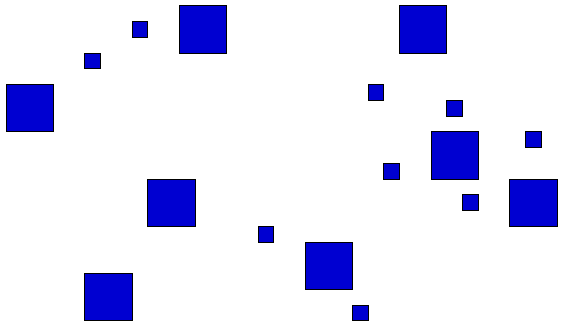
\includegraphics[width=\textwidth,keepaspectratio]{objetos1}
                \caption{Imagem original \texttt{objetos1}}
                \label{fig:objetos1-orig}
            \end{subfigure}
            \hfill
            \begin{subfigure}{0.23\textwidth}
                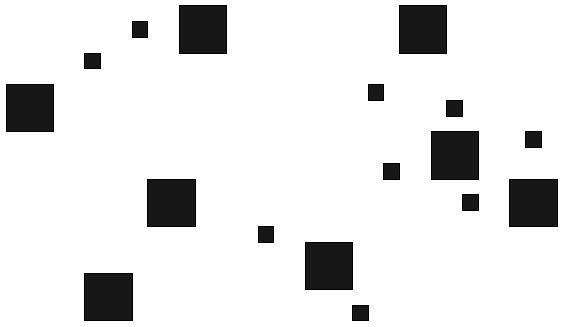
\includegraphics[width=\textwidth,keepaspectratio]{objetos1-objetos}
                \caption{Imagem monocromática \texttt{objetos1}}
                \label{fig:objetos1-mono}
            \end{subfigure}

            % objetos2
            \begin{subfigure}{0.23\textwidth}
                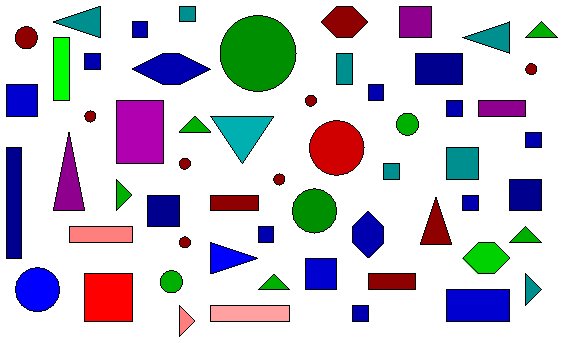
\includegraphics[width=\textwidth,keepaspectratio]{objetos2}
                \caption{Imagem original \texttt{objetos2}}
                \label{fig:objetos2-orig}
            \end{subfigure}
            \hfill
            \begin{subfigure}{0.23\textwidth}
                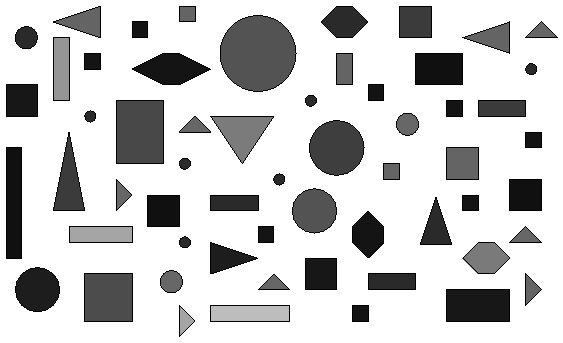
\includegraphics[width=\textwidth,keepaspectratio]{objetos2-objetos}
                \caption{Imagem monocromática \texttt{objetos2}}
                \label{fig:objetos2-mono}
            \end{subfigure}

            % objetos3
            \begin{subfigure}{0.23\textwidth}
                
\includegraphics[width=\textwidth,keepaspectratio]{objetos3}
                \caption{Imagem original \texttt{objetos3}}
                \label{fig:objetos3-orig}
            \end{subfigure}
            \hfill
            \begin{subfigure}{0.23\textwidth}
                
\includegraphics[width=\textwidth,keepaspectratio]{objetos3-objetos}
                \caption{Imagem monocromática \texttt{objetos3}}
                \label{fig:objetos3-mono}
            \end{subfigure}

            \caption{Comparativo do resultado da monocromatização}
            \label{fig:monocromatizacao}
        \end{figure}

        A monocromatização é um passo simples e os resultados coincidem com o esperado, sem perdas de objetos.

    \subsection{Rotulação e contagem}

        A rotulação realizada pelo \emph{scikit-image} é precisa, não levando em consideração nível de cinza, mas sim a conexidade dos pontos, como descrito na metodologia.

        Uma limitação do método utilizado, no entanto, é o não descarte do objeto ``fundo''. Ao contrário do enunciado do trabalho, nessa implementação, o fundo foi considerado como objeto, dado que existem casos em que seria difícil sua identificação. Por exemplo, estaríamos descartando o objeto errado ao considerarmos algumas soluções de descarte:
        \begin{itemize}
            \item Se escolhessemos o fundo pelo índice zero da lista de objetos identificados e houvesse um objeto no primeiro ponto da imagem (posição $(0, 0)$), ele possuiria índice zero;
            \item Se escolhessemos o fundo pela maior área e aplicássemos a uma imagem que possui muitos objetos (deixando pouca área ao fundo);
            \item Se escolhessemos pela cor, necessitaria de intervenção humana relativamente complexa.
        \end{itemize}

        Dessa forma, ficamos com essa limitação de considerar o fundo como objeto, mas não temos perdas de objetos errados.

        Os resultados serão apresentados posteriormente na \cref{sec:resultados-medicao}, junto com as estatísticas de cada objeto.

    \subsection{Medição de área e cálculo da centroide}

        Como descrito no método, para medição da área e cálculo da centroide, temos a solução pronta pela função \texttt{getprops} do \emph{scikit-image}. Os resultados coincidem com o apresentado no enunciado e poderão ser verificados na \cref{sec:resultados-medicao}.

    \subsection{Cálculo do perímetro e isolamento do contorno}
    \label{sec:resultados-medicao}

        Já para o cálculo do perímetro e isolamento do contorno, tivemos que isolar as regiões da imagem, uma a uma, para aplicar as funções da biblioteca.

        Salvamos a matriz isolada utilizada para cálcular o perímetro e encontrar o contorno: exemplos do isolamento são mostrados na \cref{fig:isolamento-regioes}. Temos em branco (nesta imagem binária, com valor $1$) a região selecionada (objeto) e em preto ($0$), o fundo. Todas as imagens podem ser verificadas no repositório do trabalho.

        \begin{figure}[H]
            \centering

            % objetos1
            \begin{subfigure}{0.23\textwidth}
                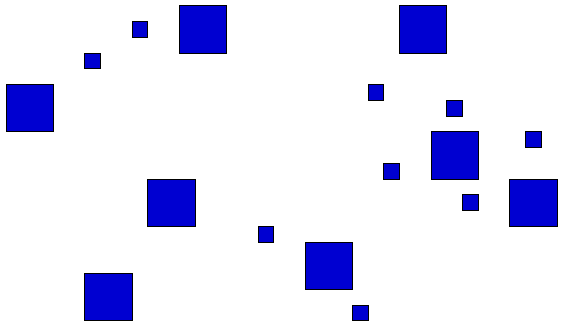
\includegraphics[width=\textwidth,keepaspectratio]{objetos1}
                \caption{Imagem original \texttt{objetos1}}
                \label{fig:objetos1-regioes-orig}
            \end{subfigure}
            \hfill
            \begin{subfigure}{0.23\textwidth}
                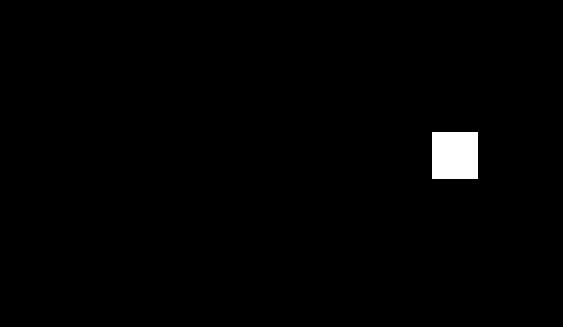
\includegraphics[width=\textwidth,keepaspectratio]{regioes/objetos1-region-9}
                \caption{Região isolada de \texttt{objetos1}}
                \label{fig:objetos1-regioes-isolada}
            \end{subfigure}

            % objetos3
            \begin{subfigure}{0.23\textwidth}
                
\includegraphics[width=\textwidth,keepaspectratio]{objetos3}
                \caption{Imagem original \texttt{objetos3}}
                \label{fig:objetos3-regioes-orig}
            \end{subfigure}
            \hfill
            \begin{subfigure}{0.23\textwidth}
                
\includegraphics[width=\textwidth,keepaspectratio]{regioes/objetos3-region-2}
                \caption{Região isolada de \texttt{objetos3}}
                \label{fig:objetos3-regioes-isolada}
            \end{subfigure}

            \caption{Exemplo de isolamento de regiões}
            \label{fig:isolamento-regioes}
        \end{figure}

        Os resultados numéricos do perímetro podem ser encontrados nas \cref{fig:resultado-objetos1,fig:resultado-objetos2,fig:resultado-objetos3}.

        \begin{figure*}
            \begin{mdframed}
                \begin{scriptsize}
                    \verbatiminput{../imgs/objetos1-stats.txt}
                \end{scriptsize}
            \end{mdframed}

            \caption{Informações numéricas de cada região da imagem \texttt{objetos1}}
            \label{fig:resultado-objetos1}
        \end{figure*}

        \begin{figure*}
            \begin{mdframed}
                \begin{scriptsize}
                    \verbatiminput{../imgs/objetos3-stats.txt}
                \end{scriptsize}
            \end{mdframed}

            \caption{Informações numéricas de cada região da imagem \texttt{objetos3}}
            \label{fig:resultado-objetos3}
        \end{figure*}

        \begin{figure*}
            \begin{mdframed}
                \begin{scriptsize}
                    \verbatiminput{../imgs/objetos2-stats.txt}
                \end{scriptsize}
            \end{mdframed}

            \caption{Informações numéricas de cada região da imagem \texttt{objetos2}}
            \label{fig:resultado-objetos2}
        \end{figure*}

        Para o contorno, a cada região foi aplicada a função \texttt{find_contours} de \emph{scikit-image}, salvamos a matriz binária resultante dessa função (onde $1$ é o contorno e $0$, o fundo) para verificação.

        Para produzir a imagem com os contornos de todas as regiões unificados, somamos todas essas matrizes de contorno (uma para cada região) em uma só matriz acumuladora. Essa matriz também foi exportada como uma imagem, podemos ver para uma região e comparar com o resultado final na \cref{fig:isolamento-contornos}.

        \begin{figure}[H]
            \centering

            % objetos1
            \begin{subfigure}{0.23\textwidth}
                
\includegraphics[width=\textwidth,keepaspectratio]{contornos/objetos1-region-9-contornos}
                \caption{Contorno de uma região de \texttt{objetos1}}
                \label{fig:objetos1-contorno-isolado}
            \end{subfigure}
            \hfill
            \begin{subfigure}{0.23\textwidth}
                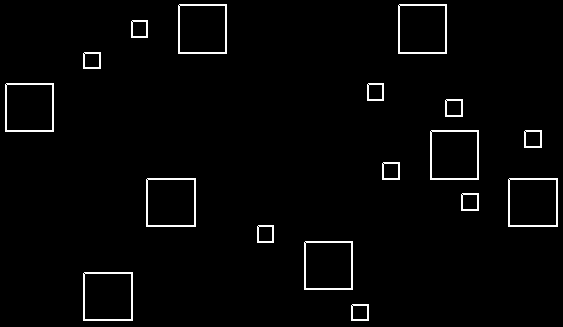
\includegraphics[width=\textwidth,keepaspectratio]{objetos1-contorno}
                \caption{Contorno de todas as regiões de \texttt{objetos1}}
                \label{fig:objetos1-contornos}
            \end{subfigure}

            % objetos2
            \begin{subfigure}{0.23\textwidth}
                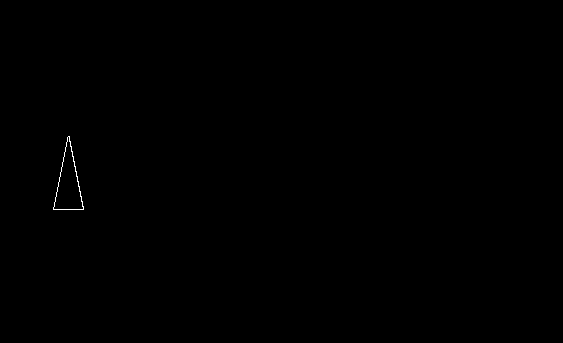
\includegraphics[width=\textwidth,keepaspectratio]{contornos/objetos2-region-29-contornos}
                \caption{Contorno de uma região de \texttt{objetos2}}
                \label{fig:objetos2-contorno-isolado}
            \end{subfigure}
            \hfill
            \begin{subfigure}{0.23\textwidth}
                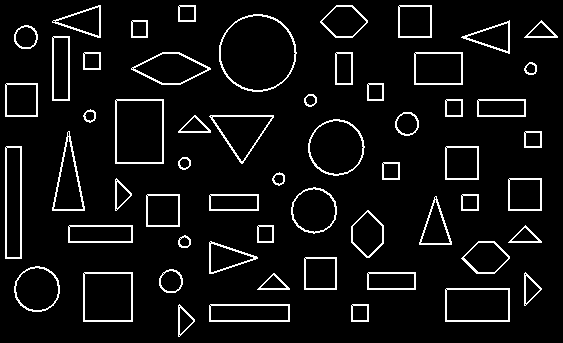
\includegraphics[width=\textwidth,keepaspectratio]{objetos2-contorno}
                \caption{Contorno de todas as regiões de \texttt{objetos2}}
                \label{fig:objetos2-contornos}
            \end{subfigure}

            % objetos3
            \begin{subfigure}{0.23\textwidth}
                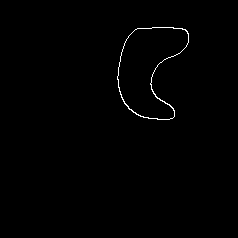
\includegraphics[width=\textwidth,keepaspectratio]{contornos/objetos3-region-2-contornos}
                \caption{Contorno de uma região de \texttt{objetos3}}
                \label{fig:objetos3-contorno-isolado}
            \end{subfigure}
            \hfill
            \begin{subfigure}{0.23\textwidth}
                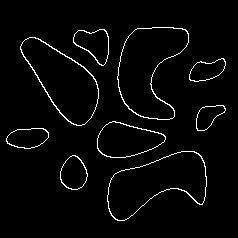
\includegraphics[width=\textwidth,keepaspectratio]{objetos3-contorno}
                \caption{Contorno de todas as regiões de \texttt{objetos3}}
                \label{fig:objetos3-contornos}
            \end{subfigure}

            \caption{Junção dos contornos das regiões}
            \label{fig:isolamento-contornos}
        \end{figure}

    \subsection{Classificação quanto área}

        Como pudemos ver nos resultados numéricos (\cref{fig:resultado-objetos1,fig:resultado-objetos2,fig:resultado-objetos3}), as regiões foram corretamente categorizadas quanto à área.

        Os histogramas produzidos pelo \emph{Matplotlib} podem ser vistos na \cref{fig:histogramas}.

        \begin{figure}[H]
            % objetos1
            \begin{subfigure}{0.48\textwidth}
                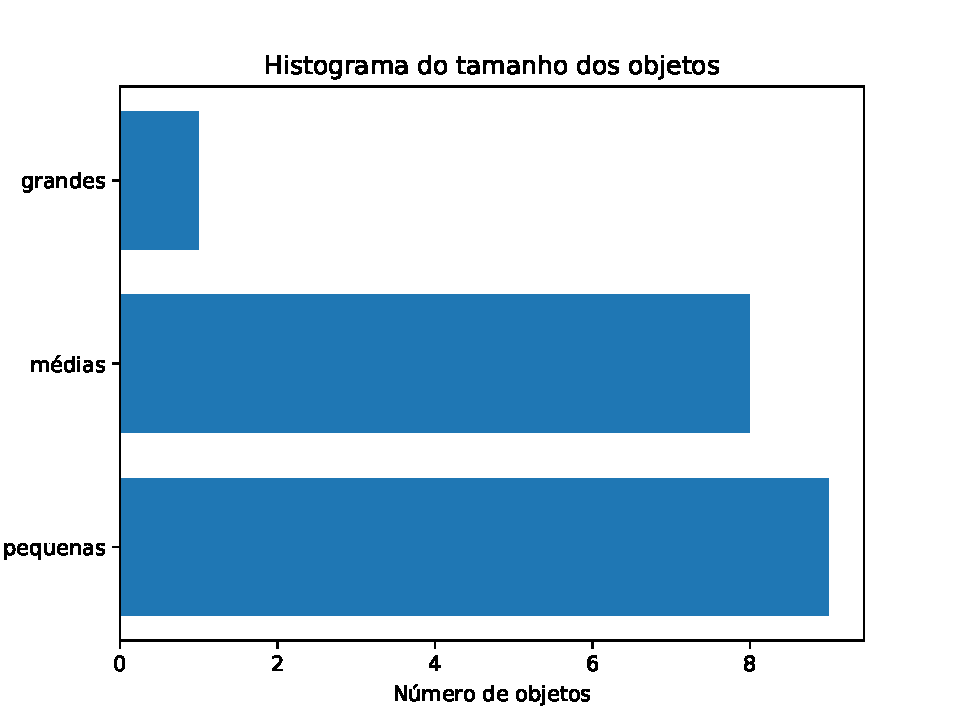
\includegraphics[width=\textwidth,keepaspectratio]{objetos1-histograma}
                \caption{Histograma de \texttt{objetos1}}
                \label{fig:objetos1-histograma}
            \end{subfigure}

            % objetos2
            \begin{subfigure}{0.48\textwidth}
                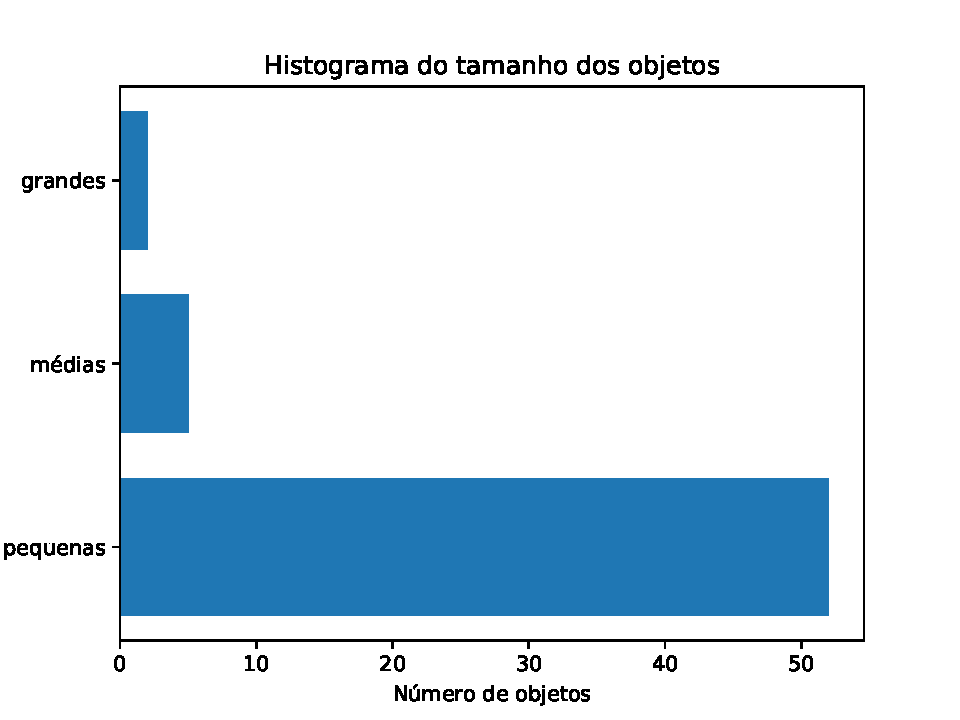
\includegraphics[width=\textwidth,keepaspectratio]{objetos2-histograma}
                \caption{Histograma de \texttt{objetos2}}
                \label{fig:objetos2-histograma}
            \end{subfigure}

            % objetos3
            \begin{subfigure}{0.48\textwidth}
                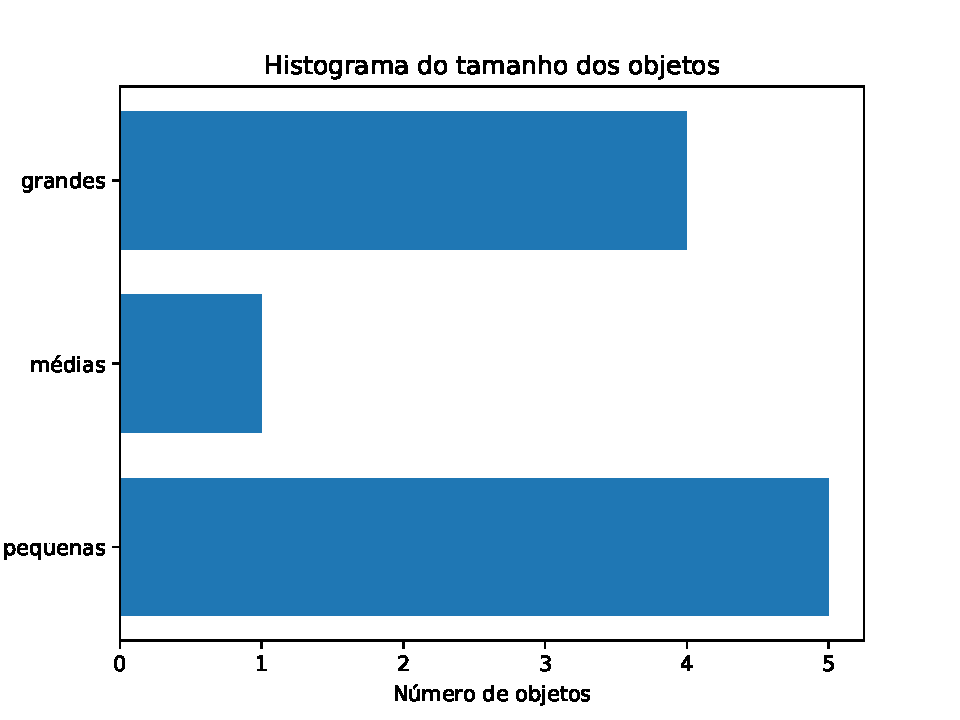
\includegraphics[width=\textwidth,keepaspectratio]{objetos3-histograma}
                \caption{Histograma de \texttt{objetos3}}
                \label{fig:objetos3-histograma}
            \end{subfigure}

            \caption{Histograma das imagens}
            \label{fig:histogramas}
        \end{figure}


\section{Conclusão}

    O trabalho mostra que, a partir de uma simplificação de uma imagem (que pode ser obtida se as condições podem ser bem controladas), é rápido determinar a área, posição e tamanho de objetos, informações muito requisitadas em automação industrial, por exemplo, para verificação.

    Com as informações obtidas, como o contorno, conseguimos comparar com o que era esperado através de funções matemáticas e/ou outros algoritmos estudados na disciplina.

    Os resultados foram bastante satisfatórios e pouca correção foi necessária para aplicação das funções já implementadas e testadas pelas bibliotecas.

\end{document}
